\documentclass[conference]{IEEEtran}
\IEEEoverridecommandlockouts
% The preceding line is only needed to identify funding in the first footnote. If that is unneeded, please comment it out.
\usepackage{cite}
\usepackage{amsmath,amssymb,amsfonts}
\usepackage[hidelinks]{hyperref}
\usepackage{algorithmic}
\usepackage{graphicx}
\usepackage{booktabs}
\usepackage{textcomp}
\usepackage{xcolor}
\def\BibTeX{{\rm B\kern-.05em{\sc i\kern-.025em b}\kern-.08em
    T\kern-.1667em\lower.7ex\hbox{E}\kern-.125emX}}
\begin{document}


\title{Composition of concrete and its influence on compressive strength\\
%{\footnotesize \textsuperscript{*}Note: Sub-titles are not captured in Xplore and
%should not be used}
%\thanks{Identify applicable funding agency here. If none, delete this.}
}

\author{\IEEEauthorblockN{Filipe P. de Farias}
\IEEEauthorblockA{\textit{Department of Teleinformatics Engineering} \\
\textit{Federal University of Ceará}\\
Fortaleza, Brazil \\
filipepfarias@fisica.ufc.br}
\and
\IEEEauthorblockN{Yvo J. M. Sales}
\IEEEauthorblockA{\textit{Department of Teleinformatics Engineering} \\
\textit{Federal University of Ceará}\\
Fortaleza, Brazil \\
yvo@gtel.ufc.br}
}

\maketitle

\begin{abstract}
The compressive strength of concrete impacts directly on its application. The difference between the concrete for columns or beams and the concrete for pavements is mainly due the compressive strength it is able to resist. In this work, we perform an unconditional and a class-conditional mono-variate analysis as well as unconditional bi-variate and multi-variate analysis of a concrete database.
\end{abstract}

\begin{IEEEkeywords}
concrete, compresive, strength, machine, learning, pre-processing
\end{IEEEkeywords}

\section{Introduction}
A material formed by aggregates bonded together by a fluid material that hardens over time has been used by humans for construction since many years ago\cite{b3}. Nowadays this material is known as concrete and it's widely used in the construction field. The aggregates used in the concrete affect directly its compressive strength which highly impacts its applications. For instance, in general, the concrete for columns or beams needs to have a greater compressive strength than the one for pavement. On this paper, we carry out an statistical analysis on a dataset extracted from the UCI Machine Learning Repository (University of California, Irvine) that collects information about the concentration of some aggregates used to form different types of concretes and their resulting compressive strenght. 

This work is divided as follows. A description of the data is given in Section \ref{data_description}. The Section \ref{data_analysis} brings an unconditional and a class-conditional mono-variate analysis as well as unconditional bi-variate and multi-variate analysis of the data. Finally, the conclusions and considerations are exposed in Section \ref{conclusions}.

% This works tries to predict this compressive strength and to classify when the concrete is proper to be applied in structures.  In the UCI database the concrete is tested with different components concentrations and different curing time (ages). 

\section{Data description}\label{data_description}

The composition of each of the $N$ concrete samples is given by the concentrations (kg/m\textsuperscript{3}) of $D$ components: Cement, Blast Furnace Slag, Fly Ash, Water, Superplasticizer, Coarse Aggregate and Fine Aggregate. Each sample has its Age (day) and the measured Concrete compressive strength (MPa), as described in Table~\ref{data_description_table}.

\begin{table}[htp]
\caption{Data description}
\begin{center}
  \begin{tabular}{@{} clc @{}}
    \toprule
    Component & Description & Unit \\ 
    \midrule
    $D_1$ & Cement & kg/m\textsuperscript{3} \\ 
    $D_2$ & Blast Furnace Slag & kg/m\textsuperscript{3} \\ 
    $D_3$ & Fly Ash & kg/m\textsuperscript{3} \\ 
    $D_4$ & Water & kg/m\textsuperscript{3} \\ 
    $D_5$ & Superplasticizer & kg/m\textsuperscript{3} \\ 
    $D_6$ & Coarse Aggregate & kg/m\textsuperscript{3} \\ 
    $D_7$ & Fine Aggregate & kg/m\textsuperscript{3} \\ 
    $D_8$ & Age & days \\ 
	\midrule
    N & 1030 samples&  \\ 
    \bottomrule
  \end{tabular}
\end{center}
\label{data_description_table}
\end{table}%

The concrete was stratified into $L=3$ classes\cite{b1}. This is, the concrete which is weak and not recommended for structures $L_1$, the \emph{Non-standard}. The concrete whose strength is in a range that can be applied to structures is classified as $L_2$, or \emph{Standard}. And the high performance concrete $L_3$, \emph{High-standard}.

The observations are the measured compressive strengths of each sample and, as the predictors $D_1 - D_7$, are continuous. The Age ($D_8$) of the concrete is extremely discrete.

\section{Data analysis}\label{data_analysis}

In order to do future works, an analysis of the data is needed to understand them and perform their validation.

\subsection{Unconditional Mono-variate Analysis}

The statistics of each predictor is obtained performing a mono-variate analysis. At this step is possible to verify how the data is distributed.

\begin{table}[htp]
\caption{Statistics summary of the predictors}
  \centering
  \begin{tabular}{@{} crrr @{}}
    \toprule
     & Mean & STD & Skewness \\ 
    \midrule
    $D_1$ & 281.16 & 104.506 & 0.50873 \\ 
    $D_2$ & 73.89 & 86.279 & 0.79955 \\ 
    $D_3$ & 54.18 & 63.997 & 0.53657 \\ 
    $D_4$ & 181.56 & 21.354 & 0.07451 \\ 
    $D_5$ & 6.20 & 5.973 & 0.90588 \\ 
    $D_6$ & 972.91 & 77.754 & 0.04016 \\ 
    $D_7$ & 773.58 & 80.176 & 0.25264 \\ 
    $D_8$ & 45.66 & 63.169 & 3.26441 \\       
    \bottomrule
  \end{tabular}
\label{statistics_table_alldataset}
\end{table}%

In Table~\ref{statistics_table_alldataset} it is possible to see that the data are not \emph{highly skewed}, but yet are needed to be normalised to zero mean and the unitary standard deviation. This can be easier shown in Figure~\ref{uncond_monovariate}.

\begin{figure}[htbp]
\centerline{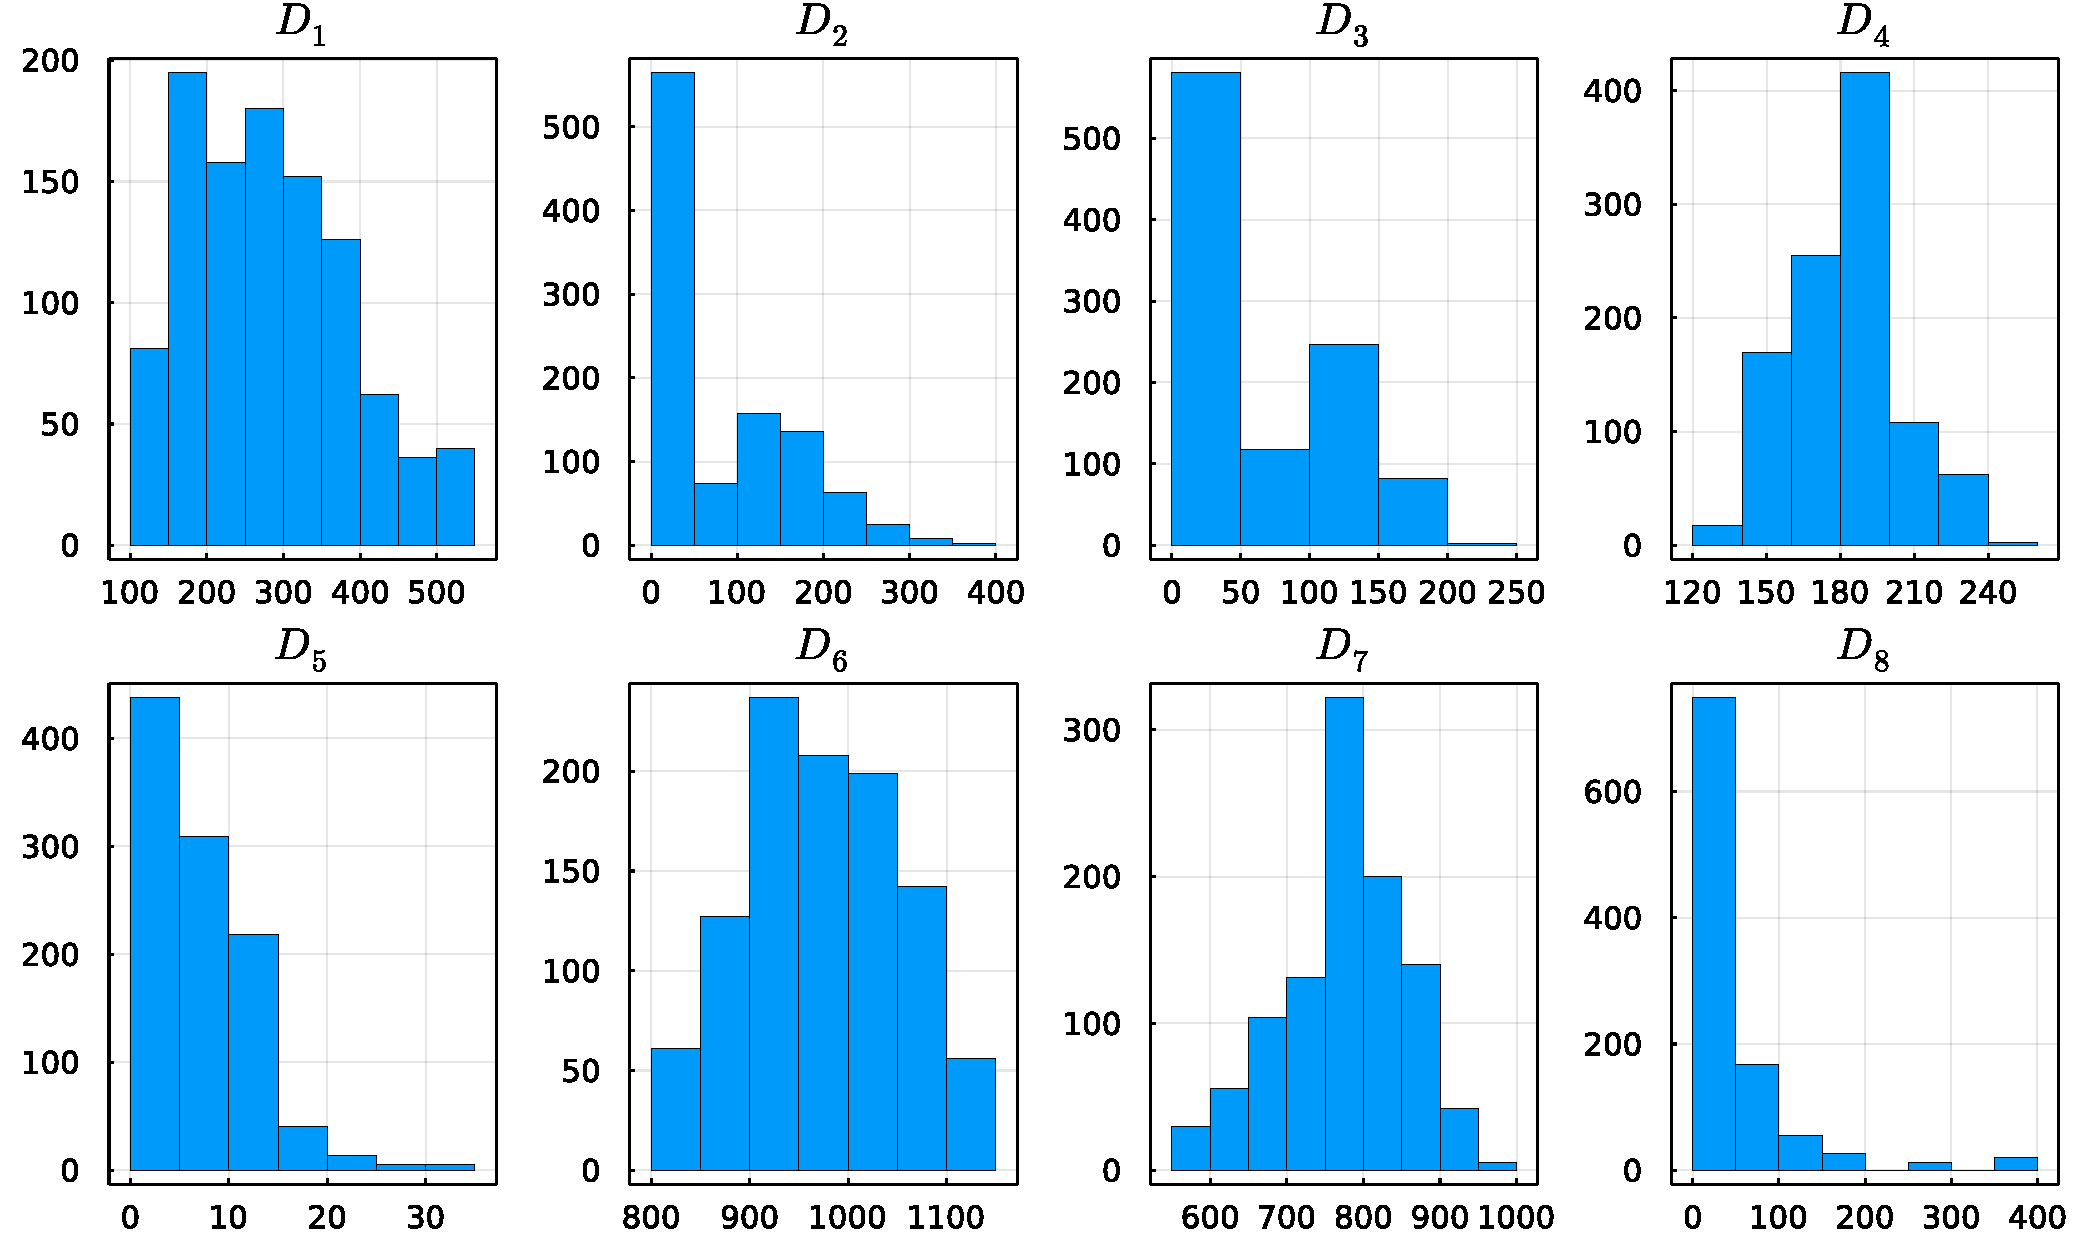
\includegraphics[width=\columnwidth]{../figures/monovariate_histograms_allcategories}}
\caption{Predictors' histograms for the unconditional monovariate analysis.}
\label{uncond_monovariate}
\end{figure}

An interesting fact is that the components that, in general, are not absent in the concrete composition has the lower skewness, as Cement, Water, Coarse and Fine Aggregates. The other components have higher skewness due to the fact they are optional in concrete mixture, thus they are allowed to have zero values in some concrete samples. Another seeable fact is the discreteness of the Age values. In general the concrete achieves the \emph{cure} at the end of 28 days. This fact explains the size of the bins in the histogram $D_8$ on Figure~\ref{uncond_monovariate} between 0 and 100. The other cure periods are sampled in dataset to test its influence in compressive strength.

\subsection{Class-conditional mono-variate analysis}

\begin{table}[htp]
  \caption{Statistics summary for class 1}
    \centering
    \begin{tabular}{@{} crrr @{}}
      \toprule
       & Mean & STD & Skewness \\ 
      \midrule
      $D_1$ & 227.649  &   77.9188  &   0.813198 \\ 
      $D_2$ & 59.1078  &  85.7506  &   1.15493 \\ 
      $D_3$ & 58.1166  &  69.7541   &  0.558909 \\ 
      $D_4$ & 185.405  &   15.7587  &  -0.933526\\ 
      $D_5$ & 3.96847  &  4.77879  &  0.781783 \\ 
      $D_6$ & 994.762   &  70.8093  &  -0.143029 \\ 
      $D_7$ & 794.88   &   66.6208  &  -0.116007 \\ 
      $D_8$ & 13.9322  &  15.9189  &   4.75222 \\       
      \bottomrule
    \end{tabular}
  \label{statistics_table_class_1}
  \end{table}%

  \begin{table}[htp]
    \caption{Statistics summary for class 2}
      \centering
      \begin{tabular}{@{} crrr @{}}
        \toprule
         & Mean & STD & Skewness \\ 
        \midrule
        $D_1$ & 277.673  &  97.8943  &  0.480469 \\ 
        $D_2$ & 75.5691 &  87.3597  &  0.793451\\ 
        $D_3$ & 57.6739 &  61.9693  &  0.330694 \\ 
        $D_4$ & 184.16   &  21.6533 &   0.16274 \\ 
        $D_5$ & 6.04743  & 5.55232  & 0.745442 \\ 
        $D_6$ & 967.124 &   75.0478  & -0.114811 \\ 
        $D_7$ & 767.236  &  82.4853 &  -0.332702 \\ 
        $D_8$ & 53.2952  & 69.2818  &  3.02584 \\       
        \bottomrule
      \end{tabular}
    \label{statistics_table_class_2}
    \end{table}%

    \begin{table}[htp]
      \caption{Statistics summary for class 3}
        \centering
        \begin{tabular}{@{} crrr @{}}
          \toprule
           & Mean & STD & Skewness \\ 
          \midrule
          $D_1$ & 365.087  &  100.273  &  -0.0967353 \\ 
          $D_2$ & 90.4862  &  81.1218  &  0.403134 \\ 
          $D_3$ & 39.9562 &   58.619   &  0.978704 \\ 
          $D_4$ & 169.694  &   23.2573  &  0.97391 \\ 
          $D_5$ & 9.73905  &  6.82741  & 0.756237 \\ 
          $D_6$ & 956.722   &  87.007  &   0.367005 \\ 
          $D_7$ & 759.52   &   86.0634  &  0.162043 \\ 
          $D_8$ & 71.1524   & 70.9618  &  2.53224 \\       
          \bottomrule
        \end{tabular}
      \label{statistics_table_class_3}
      \end{table}%


\begin{figure}[htbp]
\centerline{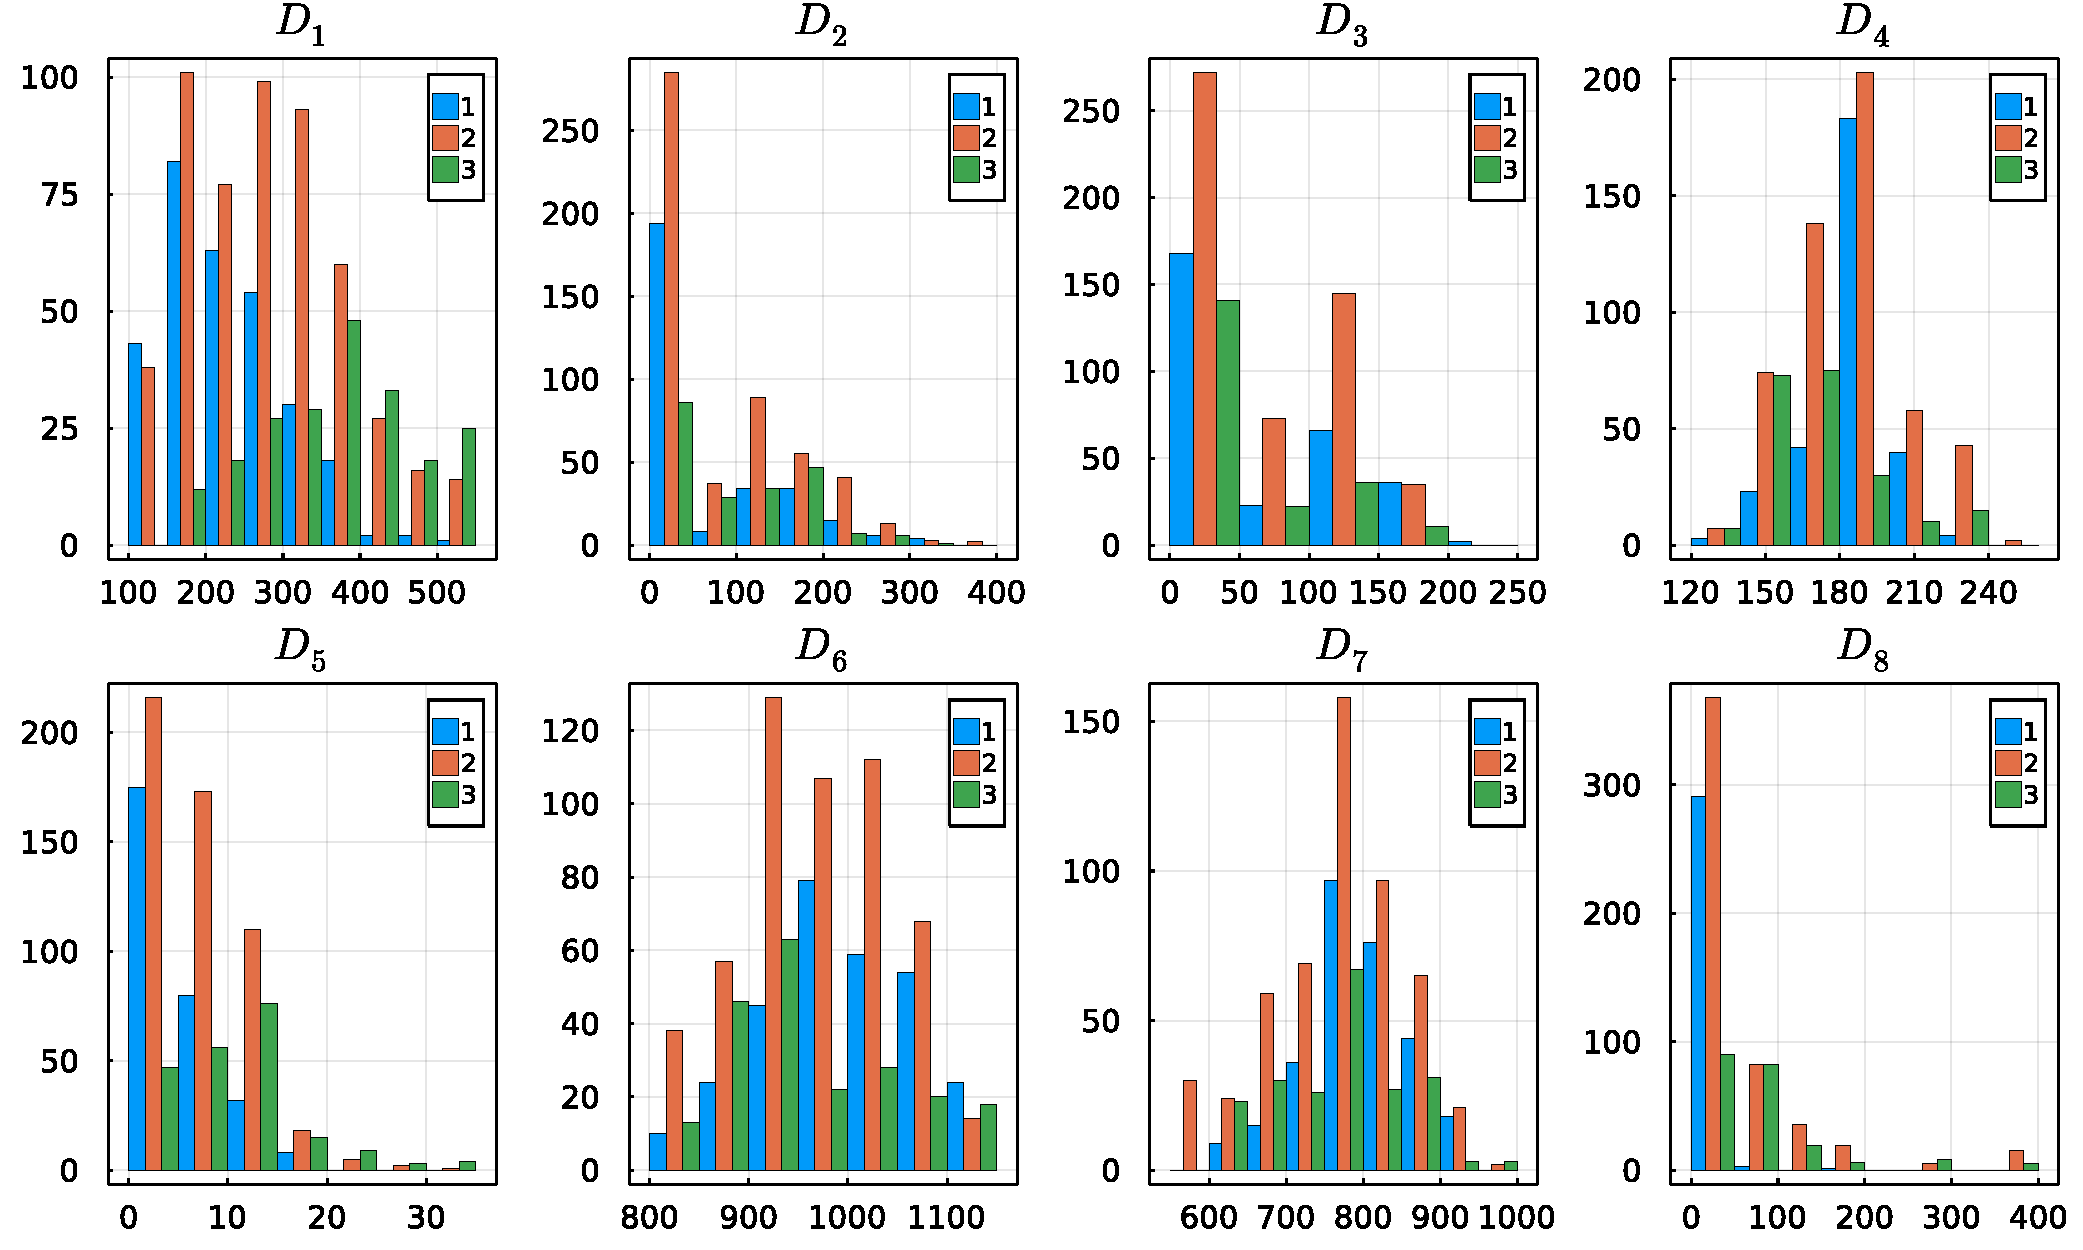
\includegraphics[width=\columnwidth]{../figures/monovariate_histograms_classcond}}
\caption{Predictors' histograms for the class-conditional monovariate analysis with each color representing a different class.}
\label{classcond_monovariate}
\end{figure}

As mentioned before, a Gaussian-like distribution can be noticed on the components except the Superplasticizer and the Age. On the other ones, as in Fly Ash, there's a large number of zeros. This behaviour is repeated on the three classes. There's no apparent discretion between the classes too. In the trial to adjust the data of each component class into a Gaussian distribution, it was noticed that a mixture model would fits better given we have exact zeros and a distribution of non zero values. This is reasonable because the zero values are the representative absence of the component.

\subsection{Unconditional bi-variate analysis}

In the pairwise comparison of the predictors, only in $(D_4,D_5)$, the Superplasticizer and Water concentrations, has a prominent negative correlation. The other predictors seemed do not have stronger correlations, as can be seen in the Figure~[\ref{corr_matrix}]. Then it was not considered eliminate predictors to simplify the problem. In the same manner mentioned before, visually it was not possible to specify a predictor that might separate the classes.

The statistics of each predictor is at Table~[].

\begin{figure}[htbp]
\centerline{\includegraphics[width=\columnwidth]{../figures/bivariate_histograms_classcond.pdf}}
\caption{Predictors' histograms and scatter plots for the unconditional bi-variate analysis with each color representing a different class.}
%\label{fig}
\end{figure}

\begin{figure}[htbp]
\centering
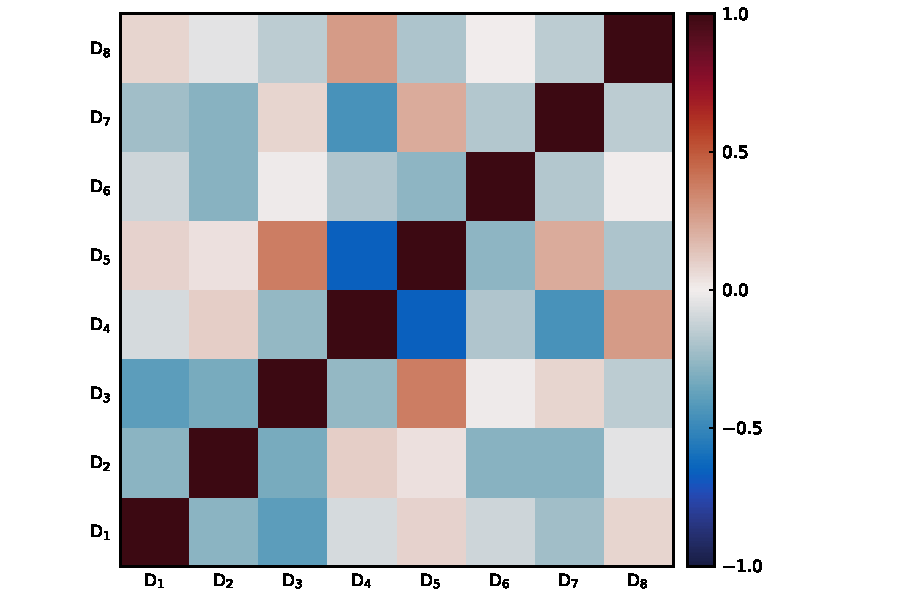
\includegraphics[width=\columnwidth,trim={0 0 60 0},clip]{../figures/predictors_corr_matrix.pdf}
\caption{Predictors' correlation matrix.}
\label{corr_matrix}
\end{figure}

\subsection{Unconditional multivariate analysis (PCA)}

How the PCs comprises the original variance is plotted on Figure~[\ref{pca_variance}]. The original predictors are projected onto the PCs space, Figure~[\ref{pca_scatter_plot}]. Note the first component, the cement $D_1$ has less information in the first two PCs components. An interesting fact about this is to know that the cement can even turns the concrete weaker to compression as long its concentration grows. The compression strength will be given by the aggregate and some chemicals, which are the predictors of major norm in the projection.

In the Figure~[\ref{pca_scatter_plot}] is shown the projection of the original data onto de first two PCs. The classes are highly overlapping and another methods are needed to allow the classes to be separeted.

\begin{figure}[htbp]
\centerline{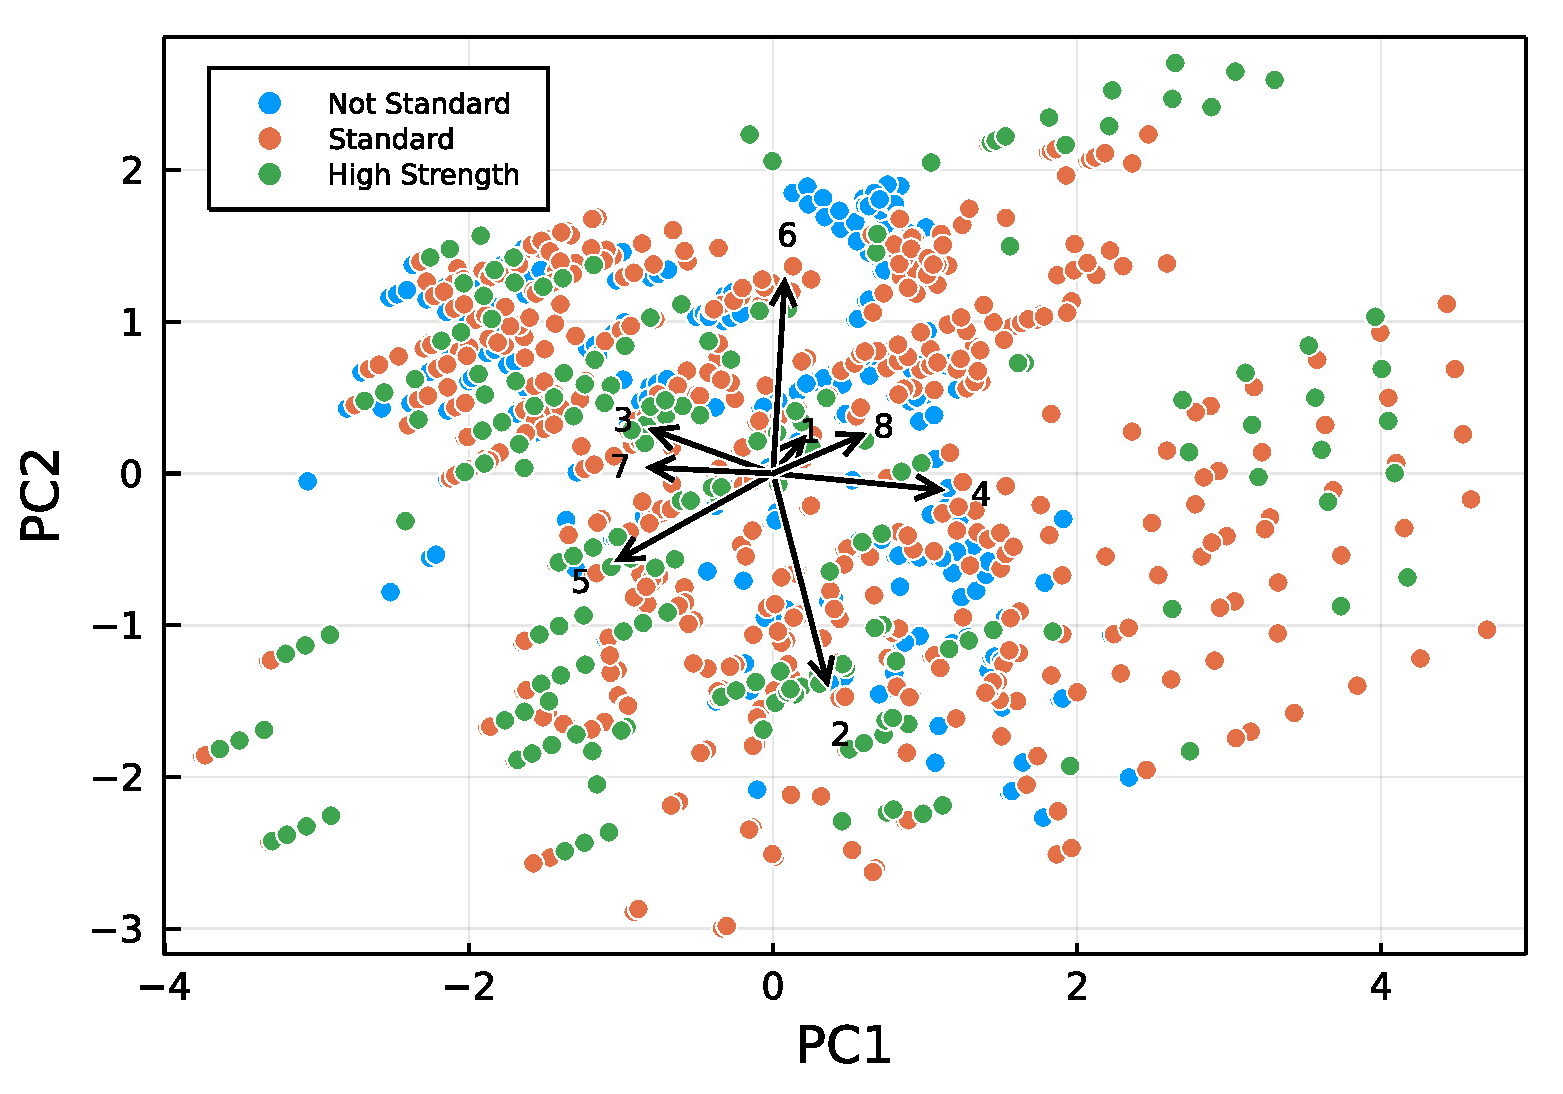
\includegraphics[width=\columnwidth]{../figures/pca_scatter_plot}}
\caption{Example of a figure caption.}
\label{pca_scatter_plot}
\end{figure}

\begin{figure}[htbp]
\centerline{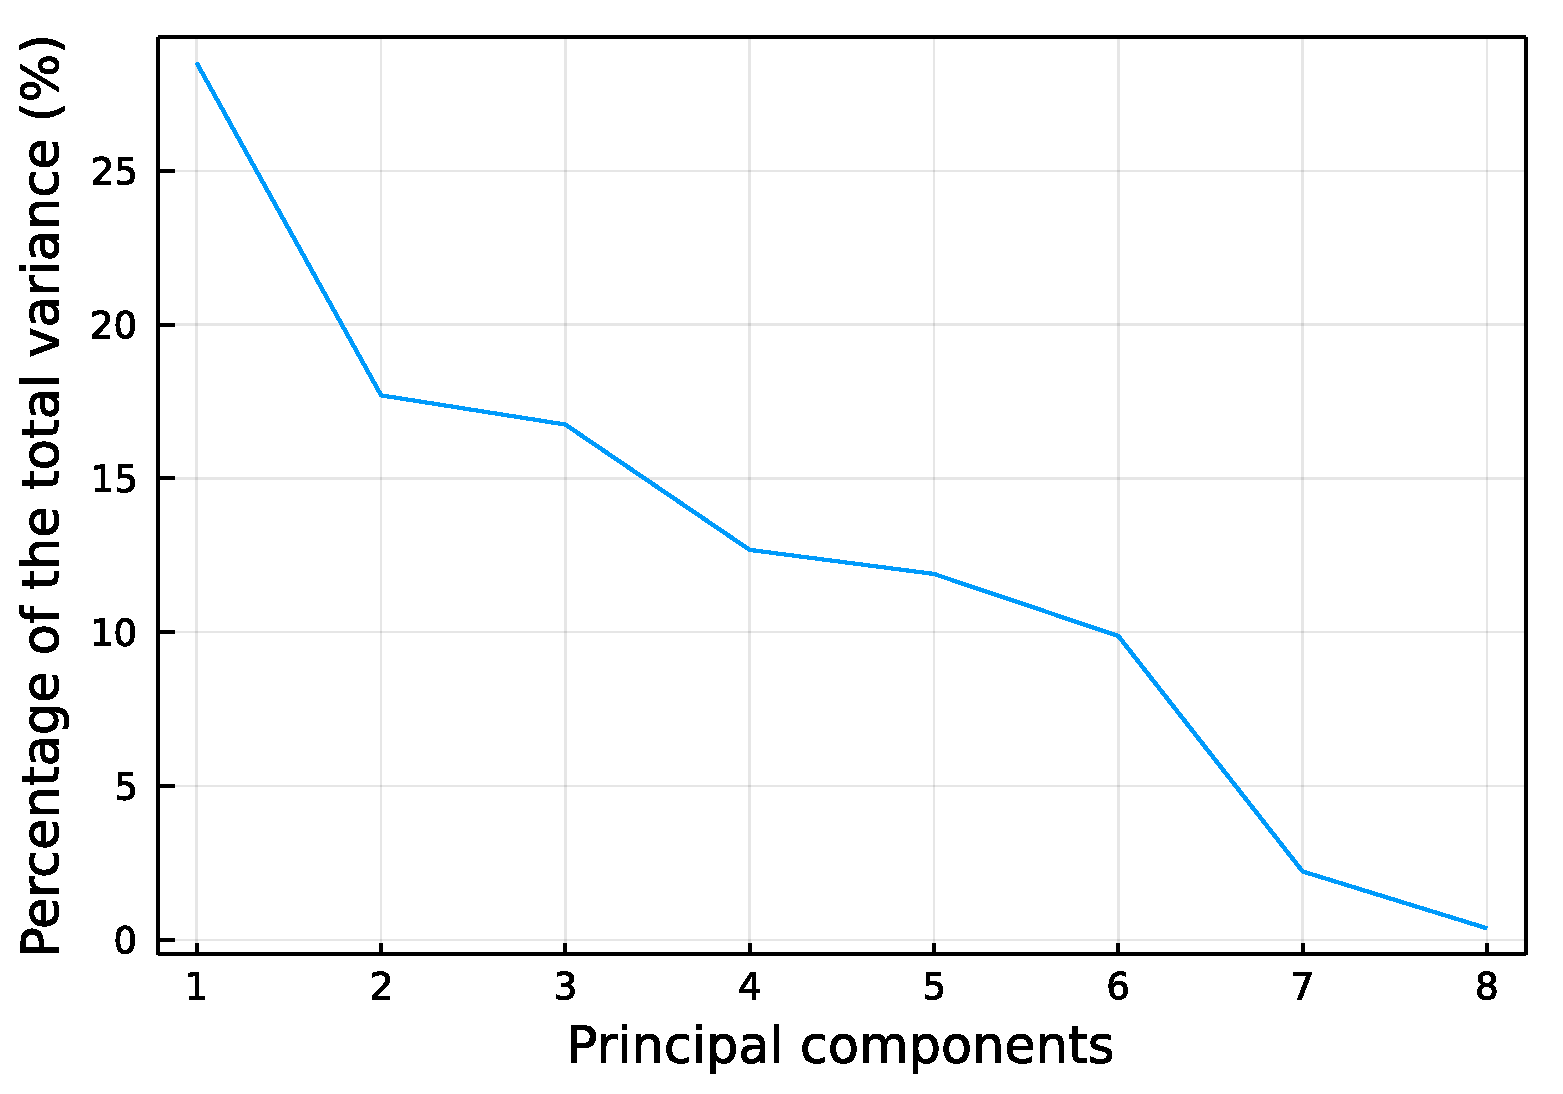
\includegraphics[width=\columnwidth]{../figures/pca_variance}}
\caption{Example of a figure caption.}
\label{pca_variance}
\end{figure}

\section{Conclusion}\label{conclusions}

The database of concrete is not easy to analyse if no knowledge about the problem of the mixture was studied. In none of the analysis the data have be shown as separable on the initially determined classes. The next step is to try to perform regression to model the compressive strength itself before trying to classify the samples.

\begin{thebibliography}{00}
\bibitem{b1} ACI Manual of Concrete Practice 2000, Part 1: Materials and General Properties of Concrete.  American Concrete Institute.  Farmington Hills, MI.
\bibitem{b2} Tibshirani, Robert, et al. The Elements of  Statistical Learning:  Data Mining, Inference, and Prediction. Alemanha, Springer New York, 2009.
\bibitem{b3} Mindess, S., and Young, J.F. Concrete. Prentice-Hall, Inc., Englewood Cliffs, NJ, 1981.
\end{thebibliography}
\end{document}